\documentclass[12pt,letterpaper]{article}
\usepackage[utf8]{inputenc}

% Ajustamos los márgenes para corregir las advertencias de fancyhdr
\usepackage[letterpaper, margin=1in, bottom=2.5in, top=1.2in]{geometry}

% Cargamos primero el paquete fancyhdr
\usepackage{fancyhdr}
% Corregimos los parámetros headheight y footskip
\setlength{\headheight}{15pt} % Al menos 14.49998pt según la advertencia
\setlength{\footskip}{72pt}   % Al menos 71.60547pt según la advertencia

\usepackage{xcolor}
\usepackage{amsmath}
\usepackage{anyfontsize}
\usepackage{graphicx}
\usepackage{tikz} % Necesario para los elementos gráficos
\usepackage{listings} % Para resaltado de sintaxis
\usepackage{sourcesanspro}
\renewcommand{\familydefault}{\sfdefault}
\usepackage{fontawesome5}
\usepackage{titlesec}
\usepackage{setspace}
\usepackage{hyperref}
\usepackage{mdframed} % Para marcos más estables

% Cargar tikz y la biblioteca de cajitas para mdframed
\usetikzlibrary{calc,shapes,positioning}

% IMPORTANT: Force the text color to be white for the entire document
\AtBeginDocument{\color{primaryColor}}

% Colors updated with better contrast
\definecolor{bgColor}{RGB}{15, 22, 36}  % Very dark blue, almost black background
\definecolor{primaryColor}{RGB}{255, 255, 255}  % White text - full white for better contrast
\definecolor{accentColor}{RGB}{255, 212, 59}  % Python Yellow
\definecolor{pythonBlue}{RGB}{120, 180, 255}  % Azul Python más claro para mejor contraste
\definecolor{secondaryColor}{RGB}{220, 230, 240}  % Lighter blue-gray for better contrast
\definecolor{terminalBg}{RGB}{22, 22, 22}  % Terminal background remains dark
\definecolor{terminalFrame}{RGB}{40, 40, 40}  % Terminal frame slightly darker
\definecolor{lineNumberColor}{RGB}{100, 100, 100}  % Color más sutil para los números de línea
\definecolor{dividerColor}{RGB}{60, 70, 90}  % Color más sutil para la línea divisoria

% Colores mejorados para el código con mayor contraste
\definecolor{codeTextColor}{RGB}{255, 255, 255}  % Blanco puro para el texto básico
\definecolor{codeKeywordColor}{RGB}{135, 206, 250}  % Azul cielo para palabras clave
\definecolor{codeCommentColor}{RGB}{144, 238, 144}  % Verde claro para comentarios
\definecolor{codeStringColor}{RGB}{255, 215, 135}  % Amarillo para strings
\definecolor{codeMethodColor}{RGB}{255, 160, 122}  % Naranja claro para métodos
\definecolor{codeFunctionColor}{RGB}{255, 215, 0}  % Dorado para funciones
\definecolor{codeNumberColor}{RGB}{255, 255, 150}  % Amarillo claro para números

% Set page background color
\pagecolor{bgColor}

% Hyperref configuration
\hypersetup{
    colorlinks=true,
    linkcolor=accentColor,
    filecolor=accentColor,
    urlcolor=accentColor,
}

% Configuración básica para listings que evita problemas con saltos de página
\lstset{
  language=Python,
  basicstyle=\normalsize\ttfamily\bfseries\color{codeTextColor}, % Tamaño reducido, en blanco y negrita
  backgroundcolor=\color{terminalBg},
  commentstyle=\color{codeCommentColor},
  keywordstyle=\color{codeKeywordColor},
  stringstyle=\color{codeStringColor},
  numberstyle=\color{lineNumberColor}, % Números de línea más sutiles
  breaklines=true,
  breakatwhitespace=true,
  tabsize=4,
  showstringspaces=false,
  frame=none,
  xleftmargin=15pt,
  xrightmargin=0pt,
  aboveskip=10pt,
  belowskip=10pt,
  numbers=left,
  numbersep=8pt,
  extendedchars=true,
  keepspaces=true,
  columns=flexible,
  lineskip=6pt, % Espacio entre líneas ligeramente reducido
  % Keywords de Python (palabras reservadas)
  morekeywords={self, yield, lambda, with, as, from, True, False, None, import, in, for, 
                if, elif, else, while, return, def, class, try, except, finally, raise, 
                break, continue, global, nonlocal, pass, assert, del},
  % Funciones incorporadas resaltadas de manera distinta
  emph={[2]print,range,sum,int,str,float,list,dict,set,tuple,next,len,type,map,filter,
         reduce,zip,enumerate,sorted,reversed,min,max,open,any,all},
  emphstyle={[2]\color{codeFunctionColor}}
}

% TERMINAL ESTILO MAC MEJORADA CON BOTONES A LA IZQUIERDA Y MENOS ESPACIO SUPERIOR
\newenvironment{macterminal}{%
    \begin{mdframed}[
        linecolor=terminalFrame,
        backgroundcolor=terminalBg,
        roundcorner=5pt,
        skipabove=10pt,
        skipbelow=10pt,
        linewidth=1pt,
        innertopmargin=10pt, % Reducido
        frametitle={%
            \tikz[baseline=(current bounding box.east), outer sep=0pt]{
                \fill[red!80!black] (0,0) circle (5pt);
                \fill[yellow!80!black] (0.7,0) circle (5pt);
                \fill[green!70!black] (1.4,0) circle (5pt);
            }
        },
        frametitlealignment=\raggedright, % Alineado a la izquierda
        frametitleaboveskip=8pt, % Espacio entre el título y el borde superior
        frametitlebelowskip=0pt, % Reducir el espacio entre el título y el contenido
    ]
    % No necesitamos más espacio vertical aquí
}{%
    \end{mdframed}%
}

% Utilities
\newcommand{\verspace}{\vspace{10pt}}

% Section styling - Esquema más elegante y mejorado contraste
\titleformat{\section}
  {\LARGE\bfseries\color{primaryColor}} % Secciones principales en blanco para mejor contraste y más grandes
  {\thesection. }
  {0pt}
  {}
  []

\titleformat{\subsection}
  {\Large\bfseries\color{accentColor}} % Subsecciones en amarillo Python y más grandes
  {\thesubsection. }
  {0pt}
  {}
  []

\titleformat{\subsubsection}
  {\large\bfseries\color{pythonBlue}} % Subsubsecciones en azul Python más claro y más grandes
  {\thesubsubsection. }
  {0pt}
  {}
  []

% Spacing for sections
\titlespacing*{\section}{0pt}{20pt}{10pt}
\titlespacing*{\subsection}{0pt}{15pt}{7pt}
\titlespacing*{\subsubsection}{0pt}{10pt}{5pt}

% Configure header and footer
\pagestyle{fancy}
\fancyhf{}

% Crear un encabezado elegante para todas las páginas (excepto la portada)
\fancyhead[L]{
    
\begin{tikzpicture}[remember picture, overlay]
        % Rectángulo de fondo para la sección Python
        \fill[pythonBlue, rounded corners=3pt] (0,0) rectangle (2.2cm,0.7cm);
        % Texto Python
        \node[text=primaryColor, font=\bfseries] at (1.1cm,0.35cm) {PYTHON};
        
        % Pequeño separador
        \fill[secondaryColor] (2.35cm,0.1cm) rectangle (2.40cm,0.6cm);
        
        % Texto Generators con el color de acento
        \node[text=accentColor, font=\bfseries, anchor=west] at (2.35cm,0.35cm) {GENERATORS};
    \end{tikzpicture}
}

% Línea de encabezado
\renewcommand{\headrulewidth}{0pt}

% Línea divisoria más sutil
\renewcommand{\footrule}{
  \vspace{0.5cm}
  \noindent\makebox[\linewidth]{\color{dividerColor}\rule{\linewidth}{0.2pt}}
  \vspace{0.5cm}
}
\renewcommand{\footrulewidth}{0.2pt}
\renewcommand{\footruleskip}{1cm}

% Configure footer with profile info
\fancyfoot[C]{
    \vspace*{0.2cm}
    \noindent
    \begin{minipage}{\textwidth}
        \begin{flushleft}
            % Profile image placeholder with TikZ
            \raisebox{0.7cm}{
            \begin{tikzpicture}[baseline]
                \path[fill=bgColor] (0,0) circle (0.8cm);
                \clip (0,0) circle (0.8cm);
                \node at (0,0) {
                    % Placeholder for profile image
                    \includegraphics[width=1.6cm,height=1.6cm]{profile-image.jpeg}
                };
            \end{tikzpicture}
            }
            \begin{minipage}[b]{0.8\textwidth}
                % Name
                {\large\bfseries\color{primaryColor}Alejandro Sánchez Yalí}
                
                % Professional description
                \par\vspace{1pt}
                {\small\color{secondaryColor}Software Developer | AI \& Blockchain Enthusiast}
                
                % Contact
                \par\vspace{1pt}
                {\small\color{accentColor}\faGlobe\hspace{5pt}\color{secondaryColor}www.asanchezyali.com}
            \end{minipage}
        \end{flushleft}
        \vspace{8pt} % Space at bottom
    \end{minipage}
}

% Estilo para la portada (sin encabezado ni pie de página)
\fancypagestyle{plain}{
    \fancyhf{}
    \renewcommand{\headrulewidth}{0pt}
    \renewcommand{\footrulewidth}{0pt}
}

% Bullet styling for lists
\renewcommand{\labelitemi}{\textcolor{accentColor}{$\bullet$}} % Primer nivel de viñetas en amarillo (mejor contraste)
\renewcommand{\labelitemii}{\textcolor{pythonBlue}{$\circ$}} % Segundo nivel de viñetas en azul

% Aumentar globalmente el tamaño de texto un 20%
\usepackage{relsize}
\AtBeginDocument{\relsize{1}} % Incrementa la fuente en aproximadamente un 20%

% Comando simplificado para la etiqueta Python
\newcommand{\languagetag}[1]{
    \begin{tikzpicture}[baseline]
        \node[fill=pythonBlue, text=primaryColor, rounded corners=5pt, inner sep=7pt] {
            {\normalsize\textbf{#1}}
        };
    \end{tikzpicture}
}

% Definir el título personalizado con alineación exacta
\newcommand{\titlepagecontents}{%
    \vspace*{6cm}
    \noindent\languagetag{Python}\\[0.4cm]
    \noindent{\fontsize{48}{52}\bfseries\color{primaryColor}Python \color{accentColor}Generators\par}
    \vspace{0.3cm}
    \noindent{\fontsize{18}{52}\color{secondaryColor}Elegant, Memory-Efficient Iterations A Powerful Python Feature\par}
    \vspace{0.3cm}
    \noindent{\color{secondaryColor}\today\par}
}

% Definir la página final similar al documento de JavaScript
\newcommand{\finalpagecontents}{%
    \vspace*{6cm}
    \begin{center}
        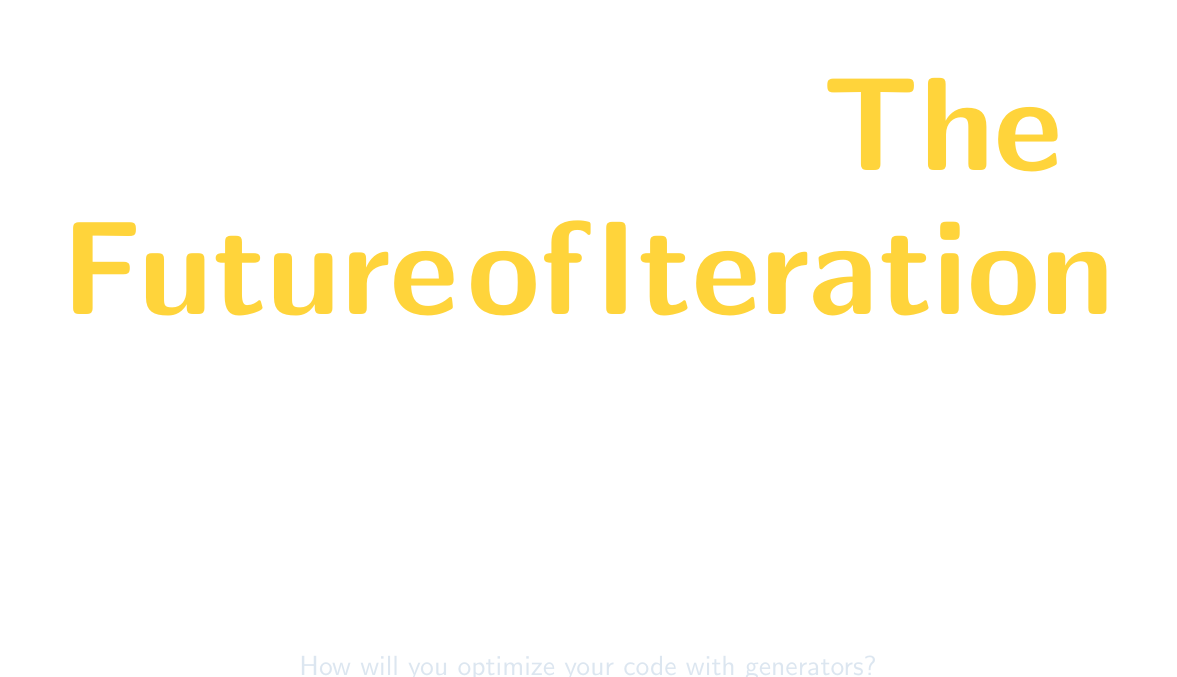
\begin{tikzpicture}
            % Title text
            \node[text width=14cm, align=center] at (0,0) {
                {\fontsize{48}{52}\bfseries\color{primaryColor}Generators: \color{accentColor}The Future of Iteration\par}
            };
            
            % Add vertical space
            \node at (0,-3) {};
            
            % Question text
            \node[text width=14cm, align=center] at (0,-6) {
                {\fontsize{22}{26}\color{secondaryColor}How will you optimize your code with generators?\par}
            };
        \end{tikzpicture}
    \end{center}
}

\begin{document}
\color{primaryColor} % Explicitly set text color to white for the entire document

\begin{titlepage}
    % Eliminamos todos los espacios adicionales para asegurar la alineación
    \titlepagecontents
\end{titlepage}

\section{Introduction to Python Generators}

Python generators provide an elegant way to create iterators with minimal memory footprint. Unlike lists that store all values in memory, generators produce values on-the-fly, making them ideal for handling large datasets or infinite sequences.

\subsection{What Are Generators?}

Generators are special functions that return an iterator using the \textbf{\textcolor{accentColor}{yield}} statement instead of \textbf{\textcolor{pythonBlue}{return}}. This allows the function to pause execution and later resume from where it left off.

\begin{itemize}
    \item \textbf{\textcolor{pythonBlue}{Memory Efficiency:}} Values are generated one at a time, not stored in memory
    \item \textbf{\textcolor{pythonBlue}{Lazy Evaluation:}} Values are computed only when needed
    \item \textbf{\textcolor{pythonBlue}{Simplicity:}} Cleaner code compared to implementing iterators manually
\end{itemize}

\subsection{Generators vs. Lists}

When comparing generators to traditional data structures like lists, we find several key differences:

\begin{itemize}
    \item \textbf{\textcolor{pythonBlue}{Memory Usage:}} Generators consume significantly less memory than equivalent lists
    \item \textbf{\textcolor{pythonBlue}{Computation:}} Lists compute all values at once; generators compute values on-demand
    \item \textbf{\textcolor{pythonBlue}{Access Patterns:}} Lists allow random access; generators only permit sequential access
    \item \textbf{\textcolor{pythonBlue}{Reusability:}} Lists can be iterated multiple times; generators are exhausted after one iteration
\end{itemize}

\section{Creating Python Generators}

There are two primary ways to create generators in Python: generator functions and generator expressions.

\subsection{Generator Functions}

Generator functions look like regular functions but use the \textbf{\textcolor{accentColor}{yield}} keyword to return values:

\begin{macterminal}
\begin{lstlisting}
def countdown(n):
    """A simple generator function that counts down from n to 1"""
    print("Starting countdown!")
    while n > 0:
        yield n
        n -= 1
    print("Countdown complete!")

# Using the generator
counter = countdown(5)
print(next(counter))  # 5
print(next(counter))  # 4
print(next(counter))  # 3
\end{lstlisting}
\end{macterminal}

The state of the function is preserved between yields, allowing it to resume execution from where it left off.

\subsection{Generator Expressions}

Generator expressions provide a concise way to create generators, similar to list comprehensions but with parentheses instead of square brackets:

\begin{macterminal}
\begin{lstlisting}
# List comprehension (creates entire list in memory)
squares_list = [x*x for x in range(1000000)]  # Uses more memory

# Generator expression (creates generator object)
squares_gen = (x*x for x in range(1000000))   # Uses minimal memory

# Using the generator expression
print(next(squares_gen))  # 0
print(next(squares_gen))  # 1
print(next(squares_gen))  # 4
\end{lstlisting}
\end{macterminal}

\section{Working with Python Generators}

Generators can be used in many contexts where iterables are expected.

\subsection{Basic Operations with Generators}

Here are common ways to interact with generators:

\begin{macterminal}
\begin{lstlisting}
def first_n_fibonacci(n):
    """Generate first n Fibonacci numbers"""
    a, b = 0, 1
    count = 0
    while count < n:
        yield a
        a, b = b, a + b
        count += 1

# Iterating with a for loop
fib = first_n_fibonacci(10)
for num in fib:
    print(num, end=' ')  # 0 1 1 2 3 5 8 13 21 34
\end{lstlisting}
\end{macterminal}

\section{Memory Efficiency with Generators}

One of the main advantages of generators is their memory efficiency.

\subsection{Memory Comparison: Lists vs. Generators}

Let's compare memory usage between lists and generators:

\begin{macterminal}
\begin{lstlisting}
import tracemalloc

# Start memory monitoring
tracemalloc.start()

# Create a large list
large_list = [i * i for i in range(1000000)]
list_snapshot = tracemalloc.take_snapshot()
list_size = sum(stat.size for stat in list_snapshot.statistics('filename'))

# Reset monitoring
tracemalloc.stop()
tracemalloc.start()

# Create an equivalent generator
large_gen = (i * i for i in range(1000000))
gen_snapshot = tracemalloc.take_snapshot()
gen_size = sum(stat.size for stat in gen_snapshot.statistics('filename'))

# Compare memory usage
print(f"List memory: {list_size / 1024 / 1024:.2f} MB")
print(f"Generator memory: {gen_size / 1024 / 1024:.2f} MB")
print(f"Memory ratio: {list_size / gen_size:.0f}x")

# Create a large list
large_list = [i * i for i in range(1000000)]
list_snapshot = tracemalloc.take_snapshot()
list_size = sum(stat.size for stat in list_snapshot.statistics('filename'))

# Reset monitoring
tracemalloc.stop()
tracemalloc.start()

# Create an equivalent generator
large_gen = (i * i for i in range(1000000))
gen_snapshot = tracemalloc.take_snapshot()
gen_size = sum(stat.size for stat in gen_snapshot.statistics('filename'))

# Compare memory usage
print(f"List memory: {list_size / 1024 / 1024:.2f} MB")
print(f"Generator memory: {gen_size / 1024 / 1024:.2f} MB")
print(f"Memory ratio: {list_size / gen_size:.0f}x")
\end{lstlisting}
\end{macterminal}

The memory savings can be substantial, especially when processing large datasets.

\section{Conclusion}

Python generators provide an elegant, memory-efficient way to work with data sequences and iterative computations. They excel in scenarios involving large datasets, stream processing, and computational pipelines.

\subsection{Key Takeaways}

\begin{itemize}
    \item \textbf{\textcolor{pythonBlue}{Memory Efficiency:}} Generators calculate values on-demand, avoiding memory overhead
    \item \textbf{\textcolor{pythonBlue}{Lazy Evaluation:}} Computation happens only when needed, improving performance
    \item \textbf{\textcolor{pythonBlue}{Elegant APIs:}} Create clean, readable code for data processing pipelines
    \item \textbf{\textcolor{pythonBlue}{Infinite Sequences:}} Work with potentially infinite data without memory concerns
    \item \textbf{\textcolor{pythonBlue}{Foundation for Async:}} Generators provided the foundation for Python's async/await syntax
\end{itemize}

Mastering generators is an essential skill for writing efficient, elegant Python code, especially when dealing with large data processing tasks.

\clearpage
\thispagestyle{empty}
\finalpagecontents

\end{document}